%! Author = mboehme
%! Date = 01.03.2023

\newpage
\section{Ergebnis}\label{sec:ergebnis}
Das Ergebnis sieht wie folgt aus:
\par\vspace{1cm}
    \centering
    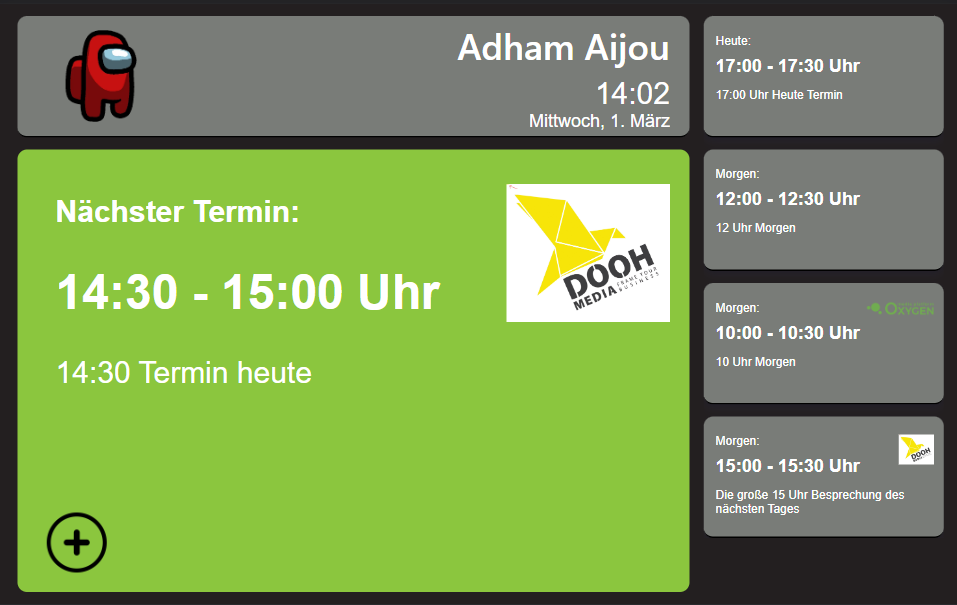
\includegraphics[width=0.8\textwidth]{Bilder/Ergebnis}
    \caption{Prototyp}
    \label{fig:Prototyp}
\par\vspace{1cm}
\raggedright
\newline
Oben links im Bild, das Bild des kleinen roten Charakters, sieht man das Logo des Gastgebers des nächsten, beziehungsweise jetzigen, Termins.
Solch ein Logo kann dargestellt werden, indem beim Erstellen des Termins, außerhalb des Tablets, bei Outlook beispielsweise, ein Bild hochgeladen wird, welches im Betreff eine bestimmte Bezeichnung enthält, die hier aus Sicherheitsgründen nicht genannt werden kann.
\newline
Die anderen Logos, sind alle Logos vom Gast des Termins.
Diese Logos können an alle Geräte gleichzeitig versendet werden, indem ein spezieller Termin erstellt wird, der nur für die Logos gedacht ist und eine einzigarte ID, sowie Befehle enthält, die dann das Bild, inklusive Firmennamen, in einer lokalen Datenbank abspeichert.
Diese Logos können hinzugefügt, gelöscht oder aktualisiert werden.
Aus Sicherheitsgründen werden die genaueren Befehle der Schnittstelle hier nicht genannt.
\newline
Es wird immer nur der erste Gast angezeigt, da das so vom Kunden gewünscht wurde.